\documentclass[1p]{elsarticle_modified}
%\bibliographystyle{elsarticle-num}

%\usepackage[colorlinks]{hyperref}
%\usepackage{abbrmath_seonhwa} %\Abb, \Ascr, \Acal ,\Abf, \Afrak
\usepackage{amsfonts}
\usepackage{amssymb}
\usepackage{amsmath}
\usepackage{amsthm}
\usepackage{scalefnt}
\usepackage{amsbsy}
\usepackage{kotex}
\usepackage{caption}
\usepackage{subfig}
\usepackage{color}
\usepackage{graphicx}
\usepackage{xcolor} %% white, black, red, green, blue, cyan, magenta, yellow
\usepackage{float}
\usepackage{setspace}
\usepackage{hyperref}

\usepackage{tikz}
\usetikzlibrary{arrows}

\usepackage{multirow}
\usepackage{array} % fixed length table
\usepackage{hhline}

%%%%%%%%%%%%%%%%%%%%%
\makeatletter
\renewcommand*\env@matrix[1][\arraystretch]{%
	\edef\arraystretch{#1}%
	\hskip -\arraycolsep
	\let\@ifnextchar\new@ifnextchar
	\array{*\c@MaxMatrixCols c}}
\makeatother %https://tex.stackexchange.com/questions/14071/how-can-i-increase-the-line-spacing-in-a-matrix
%%%%%%%%%%%%%%%

\usepackage[normalem]{ulem}

\newcommand{\msout}[1]{\ifmmode\text{\sout{\ensuremath{#1}}}\else\sout{#1}\fi}
%SOURCE: \msout is \stkout macro in https://tex.stackexchange.com/questions/20609/strikeout-in-math-mode

\newcommand{\cancel}[1]{
	\ifmmode
	{\color{red}\msout{#1}}
	\else
	{\color{red}\sout{#1}}
	\fi
}

\newcommand{\add}[1]{
	{\color{blue}\uwave{#1}}
}

\newcommand{\replace}[2]{
	\ifmmode
	{\color{red}\msout{#1}}{\color{blue}\uwave{#2}}
	\else
	{\color{red}\sout{#1}}{\color{blue}\uwave{#2}}
	\fi
}

\newcommand{\Sol}{\mathcal{S}} %segment
\newcommand{\D}{D} %diagram
\newcommand{\A}{\mathcal{A}} %arc


%%%%%%%%%%%%%%%%%%%%%%%%%%%%%5 test

\def\sl{\operatorname{\textup{SL}}(2,\Cbb)}
\def\psl{\operatorname{\textup{PSL}}(2,\Cbb)}
\def\quan{\mkern 1mu \triangleright \mkern 1mu}

\theoremstyle{definition}
\newtheorem{thm}{Theorem}[section]
\newtheorem{prop}[thm]{Proposition}
\newtheorem{lem}[thm]{Lemma}
\newtheorem{ques}[thm]{Question}
\newtheorem{cor}[thm]{Corollary}
\newtheorem{defn}[thm]{Definition}
\newtheorem{exam}[thm]{Example}
\newtheorem{rmk}[thm]{Remark}
\newtheorem{alg}[thm]{Algorithm}

\newcommand{\I}{\sqrt{-1}}
\begin{document}

%\begin{frontmatter}
%
%\title{Boundary parabolic representations of knots up to 8 crossings}
%
%%% Group authors per affiliation:
%\author{Yunhi Cho} 
%\address{Department of Mathematics, University of Seoul, Seoul, Korea}
%\ead{yhcho@uos.ac.kr}
%
%
%\author{Seonhwa Kim} %\fnref{s_kim}}
%\address{Center for Geometry and Physics, Institute for Basic Science, Pohang, 37673, Korea}
%\ead{ryeona17@ibs.re.kr}
%
%\author{Hyuk Kim}
%\address{Department of Mathematical Sciences, Seoul National University, Seoul 08826, Korea}
%\ead{hyukkim@snu.ac.kr}
%
%\author{Seokbeom Yoon}
%\address{Department of Mathematical Sciences, Seoul National University, Seoul, 08826,  Korea}
%\ead{sbyoon15@snu.ac.kr}
%
%\begin{abstract}
%We find all boundary parabolic representation of knots up to 8 crossings.
%
%\end{abstract}
%\begin{keyword}
%    \MSC[2010] 57M25 
%\end{keyword}
%
%\end{frontmatter}

%\linenumbers
%\tableofcontents
%
\newcommand\colored[1]{\textcolor{white}{\rule[-0.35ex]{0.8em}{1.4ex}}\kern-0.8em\color{red} #1}%
%\newcommand\colored[1]{\textcolor{white}{ #1}\kern-2.17ex	\textcolor{white}{ #1}\kern-1.81ex	\textcolor{white}{ #1}\kern-2.15ex\color{red}#1	}

{\Large $\underline{12n_{0840}~(K12n_{0840})}$}

\setlength{\tabcolsep}{10pt}
\renewcommand{\arraystretch}{1.6}
\vspace{1cm}\begin{tabular}{m{100pt}>{\centering\arraybackslash}m{274pt}}
\multirow{5}{120pt}{
	\centering
	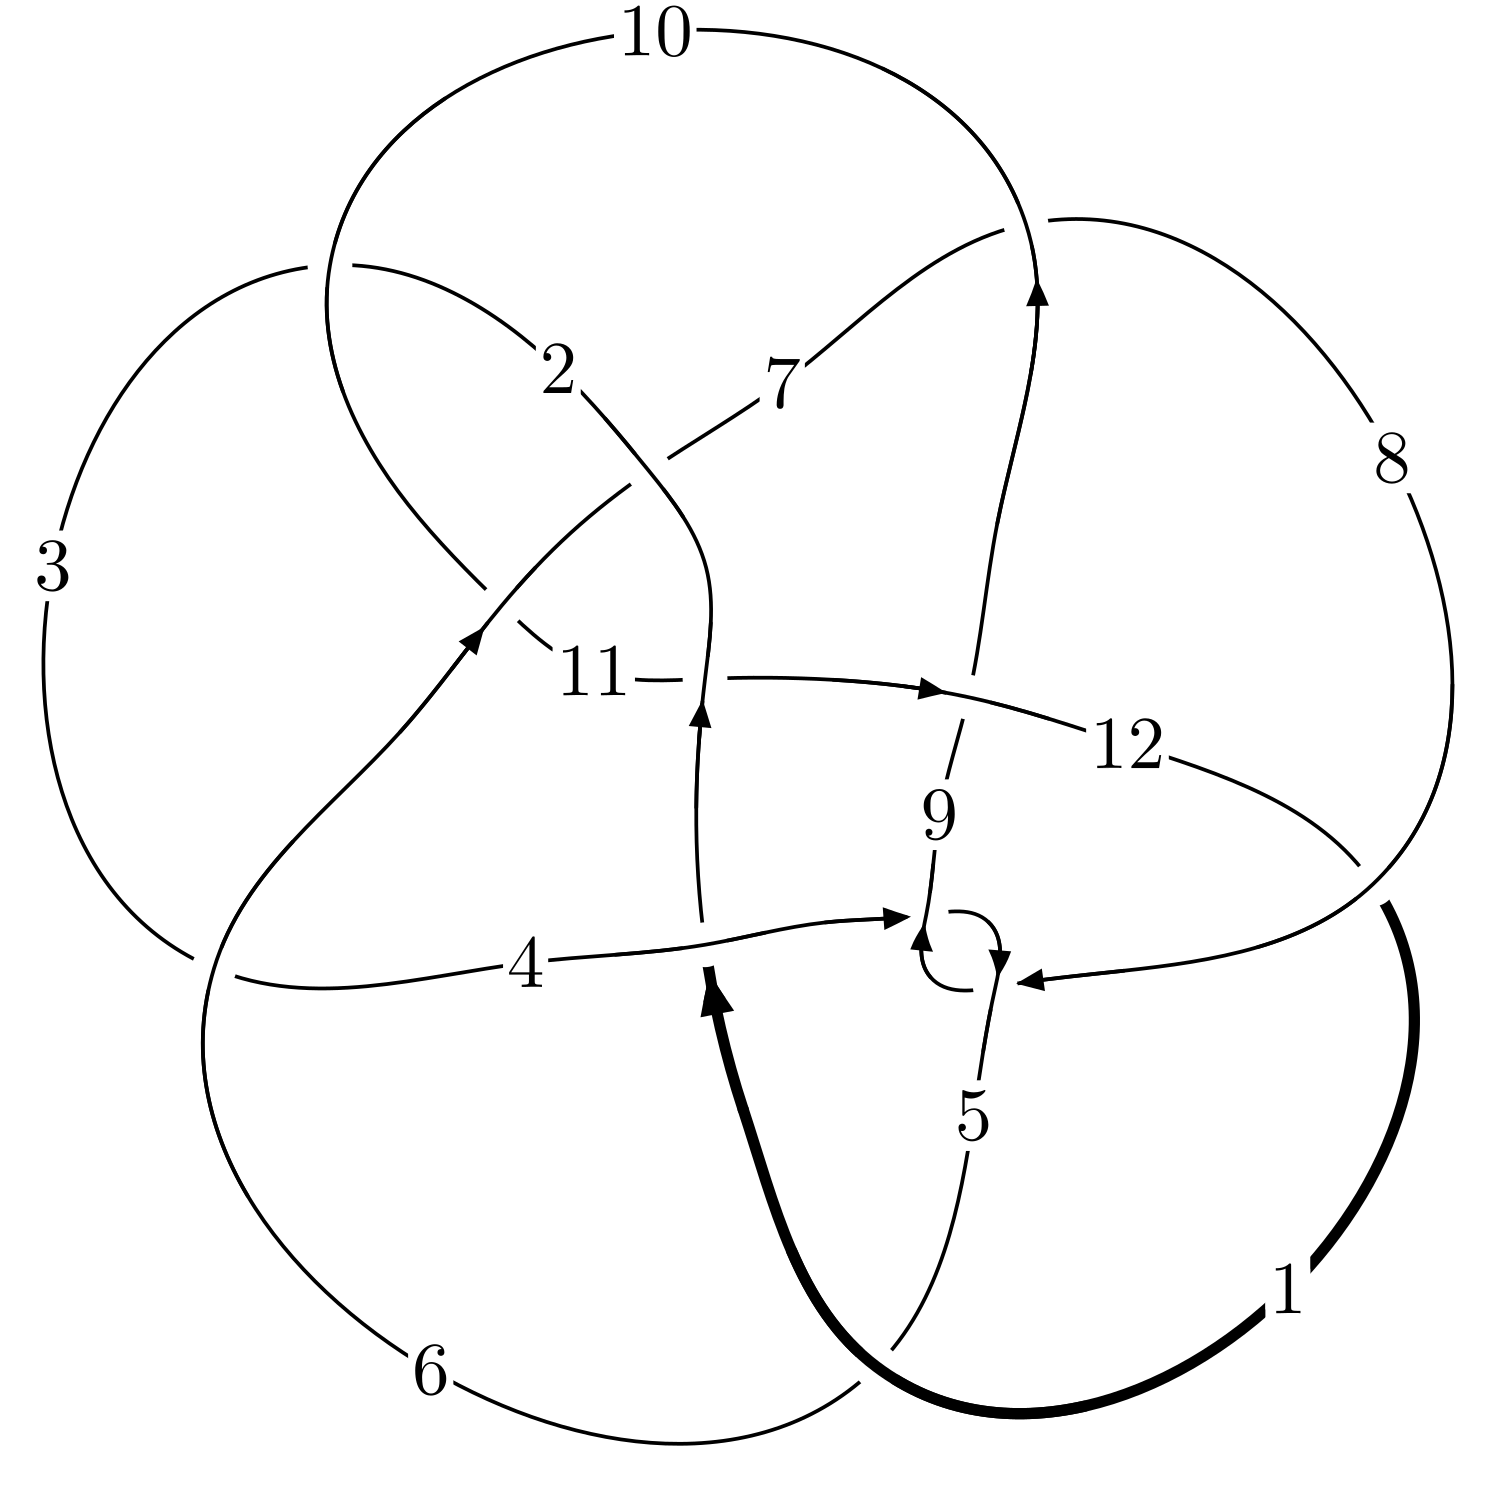
\includegraphics[width=112pt]{../../../GIT/diagram.site/Diagrams/png/2929_12n_0840.png}\\
\ \ \ A knot diagram\footnotemark}&
\allowdisplaybreaks
\textbf{Linearized knot diagam} \\
\cline{2-2}
 &
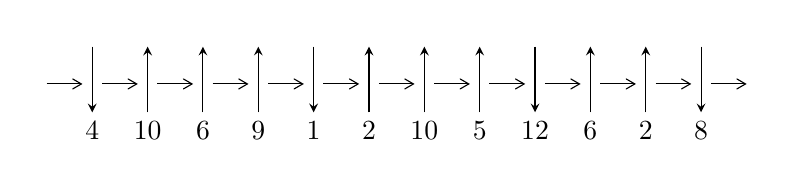
\begin{tikzpicture}[x=20pt, y=17pt]
	% nodes
	\node (C0) at (0, 0) {};
	\node (C1) at (1, 0) {};
	\node (C1U) at (1, +1) {};
	\node (C1D) at (1, -1) {4};

	\node (C2) at (2, 0) {};
	\node (C2U) at (2, +1) {};
	\node (C2D) at (2, -1) {10};

	\node (C3) at (3, 0) {};
	\node (C3U) at (3, +1) {};
	\node (C3D) at (3, -1) {6};

	\node (C4) at (4, 0) {};
	\node (C4U) at (4, +1) {};
	\node (C4D) at (4, -1) {9};

	\node (C5) at (5, 0) {};
	\node (C5U) at (5, +1) {};
	\node (C5D) at (5, -1) {1};

	\node (C6) at (6, 0) {};
	\node (C6U) at (6, +1) {};
	\node (C6D) at (6, -1) {2};

	\node (C7) at (7, 0) {};
	\node (C7U) at (7, +1) {};
	\node (C7D) at (7, -1) {10};

	\node (C8) at (8, 0) {};
	\node (C8U) at (8, +1) {};
	\node (C8D) at (8, -1) {5};

	\node (C9) at (9, 0) {};
	\node (C9U) at (9, +1) {};
	\node (C9D) at (9, -1) {12};

	\node (C10) at (10, 0) {};
	\node (C10U) at (10, +1) {};
	\node (C10D) at (10, -1) {6};

	\node (C11) at (11, 0) {};
	\node (C11U) at (11, +1) {};
	\node (C11D) at (11, -1) {2};

	\node (C12) at (12, 0) {};
	\node (C12U) at (12, +1) {};
	\node (C12D) at (12, -1) {8};
	\node (C13) at (13, 0) {};

	% arrows
	\draw[->,>={angle 60}]
	(C0) edge (C1) (C1) edge (C2) (C2) edge (C3) (C3) edge (C4) (C4) edge (C5) (C5) edge (C6) (C6) edge (C7) (C7) edge (C8) (C8) edge (C9) (C9) edge (C10) (C10) edge (C11) (C11) edge (C12) (C12) edge (C13) ;	\draw[->,>=stealth]
	(C1U) edge (C1D) (C2D) edge (C2U) (C3D) edge (C3U) (C4D) edge (C4U) (C5U) edge (C5D) (C6D) edge (C6U) (C7D) edge (C7U) (C8D) edge (C8U) (C9U) edge (C9D) (C10D) edge (C10U) (C11D) edge (C11U) (C12U) edge (C12D) ;
	\end{tikzpicture} \\
\hhline{~~} \\& 
\textbf{Solving Sequence} \\ \cline{2-2} 
 &
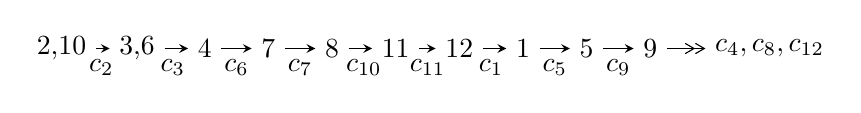
\begin{tikzpicture}[x=23pt, y=7pt]
	% node
	\node (A0) at (-1/8, 0) {2,10};
	\node (A1) at (17/16, 0) {3,6};
	\node (A2) at (17/8, 0) {4};
	\node (A3) at (25/8, 0) {7};
	\node (A4) at (33/8, 0) {8};
	\node (A5) at (41/8, 0) {11};
	\node (A6) at (49/8, 0) {12};
	\node (A7) at (57/8, 0) {1};
	\node (A8) at (65/8, 0) {5};
	\node (A9) at (73/8, 0) {9};
	\node (C1) at (1/2, -1) {$c_{2}$};
	\node (C2) at (13/8, -1) {$c_{3}$};
	\node (C3) at (21/8, -1) {$c_{6}$};
	\node (C4) at (29/8, -1) {$c_{7}$};
	\node (C5) at (37/8, -1) {$c_{10}$};
	\node (C6) at (45/8, -1) {$c_{11}$};
	\node (C7) at (53/8, -1) {$c_{1}$};
	\node (C8) at (61/8, -1) {$c_{5}$};
	\node (C9) at (69/8, -1) {$c_{9}$};
	\node (A10) at (11, 0) {$c_{4},c_{8},c_{12}$};

	% edge
	\draw[->,>=stealth]	
	(A0) edge (A1) (A1) edge (A2) (A2) edge (A3) (A3) edge (A4) (A4) edge (A5) (A5) edge (A6) (A6) edge (A7) (A7) edge (A8) (A8) edge (A9) ;
	\draw[->>,>={angle 60}]	
	(A9) edge (A10);
\end{tikzpicture} \\ 

\end{tabular} \\

\footnotetext{
The image of knot diagram is generated by the software ``\textbf{Draw programme}" developed by Andrew Bartholomew(\url{http://www.layer8.co.uk/maths/draw/index.htm\#Running-draw}), where we modified some parts for our purpose(\url{https://github.com/CATsTAILs/LinksPainter}).
}\phantom \\ \newline 
\centering \textbf{Ideals for irreducible components\footnotemark of $X_{\text{par}}$} 
 
\begin{align*}
I^u_{1}&=\langle 
-2.20855\times10^{14} u^{23}+4.72872\times10^{15} u^{22}+\cdots+1.51654\times10^{16} b+1.15899\times10^{17},\\
\phantom{I^u_{1}}&\phantom{= \langle  }9.05460\times10^{14} u^{23}-1.58566\times10^{16} u^{22}+\cdots+3.03307\times10^{16} a-3.94363\times10^{17},\\
\phantom{I^u_{1}}&\phantom{= \langle  }u^{24}-18 u^{23}+\cdots-1792 u+256\rangle \\
I^u_{2}&=\langle 
-9209872 u^{16}-47227765 u^{15}+\cdots+25630152 b+19575099,\\
\phantom{I^u_{2}}&\phantom{= \langle  }-6525033 u^{16}-41835037 u^{15}+\cdots+25630152 a-88967192,\;u^{17}+5 u^{16}+\cdots-7 u+3\rangle \\
I^u_{3}&=\langle 
50 u^{28}+444 u^{27}+\cdots+64 b+198,\;-198 u^{28} a+743 u^{28}+\cdots+3432 a-21508,\\
\phantom{I^u_{3}}&\phantom{= \langle  }u^{29}+10 u^{28}+\cdots-32 u-2\rangle \\
I^u_{4}&=\langle 
a u+b+u-1,\;6 a^2+3 a u+6 a+2 u-1,\;u^2+2\rangle \\
\\
I^v_{1}&=\langle 
a,\;b+v,\;v^2- v+1\rangle \\
\end{align*}
\raggedright * 5 irreducible components of $\dim_{\mathbb{C}}=0$, with total 105 representations.\\
\footnotetext{All coefficients of polynomials are rational numbers. But the coefficients are sometimes approximated in decimal forms when there is not enough margin.}
\newpage
\renewcommand{\arraystretch}{1}
\centering \section*{I. $I^u_{1}= \langle -2.21\times10^{14} u^{23}+4.73\times10^{15} u^{22}+\cdots+1.52\times10^{16} b+1.16\times10^{17},\;9.05\times10^{14} u^{23}-1.59\times10^{16} u^{22}+\cdots+3.03\times10^{16} a-3.94\times10^{17},\;u^{24}-18 u^{23}+\cdots-1792 u+256 \rangle$}
\flushleft \textbf{(i) Arc colorings}\\
\begin{tabular}{m{7pt} m{180pt} m{7pt} m{180pt} }
\flushright $a_{2}=$&$\begin{pmatrix}1\\0\end{pmatrix}$ \\
\flushright $a_{10}=$&$\begin{pmatrix}0\\u\end{pmatrix}$ \\
\flushright $a_{3}=$&$\begin{pmatrix}1\\- u^2\end{pmatrix}$ \\
\flushright $a_{6}=$&$\begin{pmatrix}-0.0298529 u^{23}+0.522789 u^{22}+\cdots-64.9055 u+13.0021\\0.0145631 u^{23}-0.311811 u^{22}+\cdots+40.4943 u-7.64234\end{pmatrix}$ \\
\flushright $a_{4}=$&$\begin{pmatrix}-0.00905264 u^{23}+0.149935 u^{22}+\cdots-33.0279 u+6.96109\\0.0130124 u^{23}-0.201731 u^{22}+\cdots+10.2612 u-2.31748\end{pmatrix}$ \\
\flushright $a_{7}=$&$\begin{pmatrix}-0.0152898 u^{23}+0.210978 u^{22}+\cdots-24.4112 u+5.35977\\0.0145631 u^{23}-0.311811 u^{22}+\cdots+40.4943 u-7.64234\end{pmatrix}$ \\
\flushright $a_{8}=$&$\begin{pmatrix}-0.0152898 u^{23}+0.210978 u^{22}+\cdots-24.4112 u+5.35977\\0.205024 u^{23}-3.31073 u^{22}+\cdots+151.694 u-24.0872\end{pmatrix}$ \\
\flushright $a_{11}=$&$\begin{pmatrix}-0.0521967 u^{23}+0.896396 u^{22}+\cdots-107.241 u+19.3234\\0.0431440 u^{23}-0.746461 u^{22}+\cdots+75.2130 u-13.3623\end{pmatrix}$ \\
\flushright $a_{12}=$&$\begin{pmatrix}-0.00905264 u^{23}+0.149935 u^{22}+\cdots-32.0279 u+5.96109\\0.0431440 u^{23}-0.746461 u^{22}+\cdots+75.2130 u-13.3623\end{pmatrix}$ \\
\flushright $a_{1}=$&$\begin{pmatrix}-0.00666547 u^{23}+0.0871674 u^{22}+\cdots-0.179325 u+0.846328\\0.0610145 u^{23}-0.974137 u^{22}+\cdots+45.9929 u-6.69328\end{pmatrix}$ \\
\flushright $a_{5}=$&$\begin{pmatrix}0.0545990 u^{23}-0.928564 u^{22}+\cdots+37.7724 u-3.48734\\0.146921 u^{23}-2.29092 u^{22}+\cdots+73.7072 u-11.6542\end{pmatrix}$ \\
\flushright $a_{9}=$&$\begin{pmatrix}-0.0261456 u^{23}+0.409607 u^{22}+\cdots-10.9189 u+0.860033\\0.0481684 u^{23}-0.847385 u^{22}+\cdots+96.6167 u-15.6932\end{pmatrix}$\\&\end{tabular}
\flushleft \textbf{(ii) Obstruction class $= -1$}\\~\\
\flushleft \textbf{(iii) Cusp Shapes $= -\frac{261339848863265}{1421751842414568} u^{23}+\frac{151465938324859}{50776851514806} u^{22}+\cdots-\frac{76152219280730}{533690631537} u+\frac{3978648810812680}{177718980301821}$}\\~\\
\newpage\renewcommand{\arraystretch}{1}
\flushleft \textbf{(iv) u-Polynomials at the component}\newline \\
\begin{tabular}{m{50pt}|m{274pt}}
Crossings & \hspace{64pt}u-Polynomials at each crossing \\
\hline $$\begin{aligned}c_{1},c_{9}\end{aligned}$$&$\begin{aligned}
&u^{24}-3 u^{23}+\cdots-12 u+3
\end{aligned}$\\
\hline $$\begin{aligned}c_{2}\end{aligned}$$&$\begin{aligned}
&u^{24}-18 u^{23}+\cdots-1792 u+256
\end{aligned}$\\
\hline $$\begin{aligned}c_{3},c_{7}\end{aligned}$$&$\begin{aligned}
&u^{24}+2 u^{23}+\cdots+9 u-3
\end{aligned}$\\
\hline $$\begin{aligned}c_{4},c_{8}\end{aligned}$$&$\begin{aligned}
&u^{24}-9 u^{23}+\cdots+44 u-8
\end{aligned}$\\
\hline $$\begin{aligned}c_{5},c_{12}\end{aligned}$$&$\begin{aligned}
&3(3 u^{24}+3 u^{23}+\cdots-6 u+1)
\end{aligned}$\\
\hline $$\begin{aligned}c_{6},c_{10}\end{aligned}$$&$\begin{aligned}
&3(3 u^{24}-3 u^{23}+\cdots- u-1)
\end{aligned}$\\
\hline $$\begin{aligned}c_{11}\end{aligned}$$&$\begin{aligned}
&9(9 u^{24}+141 u^{23}+\cdots+14728 u+1960)
\end{aligned}$\\
\hline
\end{tabular}\\~\\
\newpage\renewcommand{\arraystretch}{1}
\flushleft \textbf{(v) Riley Polynomials at the component}\newline \\
\begin{tabular}{m{50pt}|m{274pt}}
Crossings & \hspace{64pt}Riley Polynomials at each crossing \\
\hline $$\begin{aligned}c_{1},c_{9}\end{aligned}$$&$\begin{aligned}
&y^{24}+3 y^{23}+\cdots+66 y+9
\end{aligned}$\\
\hline $$\begin{aligned}c_{2}\end{aligned}$$&$\begin{aligned}
&y^{24}-18 y^{23}+\cdots+262144 y+65536
\end{aligned}$\\
\hline $$\begin{aligned}c_{3},c_{7}\end{aligned}$$&$\begin{aligned}
&y^{24}-20 y^{23}+\cdots+57 y+9
\end{aligned}$\\
\hline $$\begin{aligned}c_{4},c_{8}\end{aligned}$$&$\begin{aligned}
&y^{24}+11 y^{23}+\cdots+176 y+64
\end{aligned}$\\
\hline $$\begin{aligned}c_{5},c_{12}\end{aligned}$$&$\begin{aligned}
&9(9 y^{24}-87 y^{23}+\cdots-66 y+1)
\end{aligned}$\\
\hline $$\begin{aligned}c_{6},c_{10}\end{aligned}$$&$\begin{aligned}
&9(9 y^{24}-303 y^{23}+\cdots-17 y+1)
\end{aligned}$\\
\hline $$\begin{aligned}c_{11}\end{aligned}$$&$\begin{aligned}
&81(81 y^{24}-369 y^{23}+\cdots+1.23041\times10^{7} y+3841600)
\end{aligned}$\\
\hline
\end{tabular}\\~\\
\newpage\flushleft \textbf{(vi) Complex Volumes and Cusp Shapes}
$$\begin{array}{c|c|c}  
\text{Solutions to }I^u_{1}& \I (\text{vol} + \sqrt{-1}CS) & \text{Cusp shape}\\
 \hline 
\begin{aligned}
u &= \phantom{-}0.530777 + 0.640777 I \\
a &= \phantom{-}0.265857 + 0.440018 I \\
b &= \phantom{-}0.140843 - 0.403906 I\end{aligned}
 & \phantom{-}0.26899 + 1.49716 I & \phantom{-}3.11954 - 2.07751 I \\ \hline\begin{aligned}
u &= \phantom{-}0.530777 - 0.640777 I \\
a &= \phantom{-}0.265857 - 0.440018 I \\
b &= \phantom{-}0.140843 + 0.403906 I\end{aligned}
 & \phantom{-}0.26899 - 1.49716 I & \phantom{-}3.11954 + 2.07751 I \\ \hline\begin{aligned}
u &= \phantom{-}0.688395 + 1.068310 I \\
a &= \phantom{-}0.206159 - 0.248091 I \\
b &= -0.406957 - 0.049457 I\end{aligned}
 & -1.49200 + 3.53503 I & \phantom{-}6.33355 - 5.98826 I \\ \hline\begin{aligned}
u &= \phantom{-}0.688395 - 1.068310 I \\
a &= \phantom{-}0.206159 + 0.248091 I \\
b &= -0.406957 + 0.049457 I\end{aligned}
 & -1.49200 - 3.53503 I & \phantom{-}6.33355 + 5.98826 I \\ \hline\begin{aligned}
u &= -0.154209 + 1.284530 I \\
a &= -0.262592 + 0.372209 I \\
b &= \phantom{-}0.437620 + 0.394705 I\end{aligned}
 & -5.06511 + 1.65286 I & -0.70806 - 3.88591 I \\ \hline\begin{aligned}
u &= -0.154209 - 1.284530 I \\
a &= -0.262592 - 0.372209 I \\
b &= \phantom{-}0.437620 - 0.394705 I\end{aligned}
 & -5.06511 - 1.65286 I & -0.70806 + 3.88591 I \\ \hline\begin{aligned}
u &= \phantom{-}1.278810 + 0.409856 I \\
a &= -0.843748 + 0.488093 I \\
b &= \phantom{-}1.279040 - 0.278361 I\end{aligned}
 & \phantom{-}0.75060 + 2.39087 I & \phantom{-}2.55581 - 0.50009 I \\ \hline\begin{aligned}
u &= \phantom{-}1.278810 - 0.409856 I \\
a &= -0.843748 - 0.488093 I \\
b &= \phantom{-}1.279040 + 0.278361 I\end{aligned}
 & \phantom{-}0.75060 - 2.39087 I & \phantom{-}2.55581 + 0.50009 I \\ \hline\begin{aligned}
u &= \phantom{-}1.42403\phantom{ +0.000000I} \\
a &= \phantom{-}1.18251\phantom{ +0.000000I} \\
b &= -1.68393\phantom{ +0.000000I}\end{aligned}
 & \phantom{-}3.38392\phantom{ +0.000000I} & \phantom{-}2.10530\phantom{ +0.000000I} \\ \hline\begin{aligned}
u &= -0.376695 + 0.432151 I \\
a &= \phantom{-}0.796902 + 0.859648 I \\
b &= \phantom{-}0.671687 - 0.020557 I\end{aligned}
 & -0.73124 + 4.01940 I & \phantom{-}4.26636 - 3.12077 I\\
 \hline 
 \end{array}$$\newpage$$\begin{array}{c|c|c}  
\text{Solutions to }I^u_{1}& \I (\text{vol} + \sqrt{-1}CS) & \text{Cusp shape}\\
 \hline 
\begin{aligned}
u &= -0.376695 - 0.432151 I \\
a &= \phantom{-}0.796902 - 0.859648 I \\
b &= \phantom{-}0.671687 + 0.020557 I\end{aligned}
 & -0.73124 - 4.01940 I & \phantom{-}4.26636 + 3.12077 I \\ \hline\begin{aligned}
u &= -0.38587 + 1.39561 I \\
a &= \phantom{-}0.132291 - 0.512227 I \\
b &= -0.663821 - 0.382280 I\end{aligned}
 & \phantom{-}1.35141 - 3.47627 I & \phantom{-}4.76400 + 8.33538 I \\ \hline\begin{aligned}
u &= -0.38587 - 1.39561 I \\
a &= \phantom{-}0.132291 + 0.512227 I \\
b &= -0.663821 + 0.382280 I\end{aligned}
 & \phantom{-}1.35141 + 3.47627 I & \phantom{-}4.76400 - 8.33538 I \\ \hline\begin{aligned}
u &= \phantom{-}0.298932 + 0.404251 I \\
a &= \phantom{-}0.38457 - 1.82839 I \\
b &= -0.854090 + 0.391104 I\end{aligned}
 & \phantom{-}1.36425 - 1.12274 I & \phantom{-}2.97626 + 1.52454 I \\ \hline\begin{aligned}
u &= \phantom{-}0.298932 - 0.404251 I \\
a &= \phantom{-}0.38457 + 1.82839 I \\
b &= -0.854090 - 0.391104 I\end{aligned}
 & \phantom{-}1.36425 + 1.12274 I & \phantom{-}2.97626 - 1.52454 I \\ \hline\begin{aligned}
u &= -0.44722 + 1.43798 I \\
a &= -0.070696 + 0.446274 I \\
b &= \phantom{-}0.610116 + 0.301240 I\end{aligned}
 & -2.42080 - 9.85876 I & \phantom{-}4.00000 + 7.00757 I \\ \hline\begin{aligned}
u &= -0.44722 - 1.43798 I \\
a &= -0.070696 - 0.446274 I \\
b &= \phantom{-}0.610116 - 0.301240 I\end{aligned}
 & -2.42080 + 9.85876 I & \phantom{-}4.00000 - 7.00757 I \\ \hline\begin{aligned}
u &= \phantom{-}1.83440 + 0.51876 I \\
a &= \phantom{-}1.046860 - 0.052839 I \\
b &= -1.94776 - 0.44614 I\end{aligned}
 & \phantom{-}5.0719 + 17.4667 I & \phantom{-0.000000 } 0. - 8.41645 I \\ \hline\begin{aligned}
u &= \phantom{-}1.83440 - 0.51876 I \\
a &= \phantom{-}1.046860 + 0.052839 I \\
b &= -1.94776 + 0.44614 I\end{aligned}
 & \phantom{-}5.0719 - 17.4667 I & \phantom{-0.000000 -}0. + 8.41645 I \\ \hline\begin{aligned}
u &= \phantom{-}1.84303 + 0.56018 I \\
a &= -1.017100 + 0.103953 I \\
b &= \phantom{-}1.93278 + 0.37817 I\end{aligned}
 & \phantom{-}8.5754 + 11.2460 I & \phantom{-0.000000 } 0\\
 \hline 
 \end{array}$$\newpage$$\begin{array}{c|c|c}  
\text{Solutions to }I^u_{1}& \I (\text{vol} + \sqrt{-1}CS) & \text{Cusp shape}\\
 \hline 
\begin{aligned}
u &= \phantom{-}1.84303 - 0.56018 I \\
a &= -1.017100 - 0.103953 I \\
b &= \phantom{-}1.93278 - 0.37817 I\end{aligned}
 & \phantom{-}8.5754 - 11.2460 I & \phantom{-0.000000 } 0 \\ \hline\begin{aligned}
u &= \phantom{-}1.94698 + 0.52145 I \\
a &= \phantom{-}0.908100 - 0.084492 I \\
b &= -1.81211 - 0.30903 I\end{aligned}
 & \phantom{-}2.43712 + 5.84189 I & \phantom{-0.000000 } 0 \\ \hline\begin{aligned}
u &= \phantom{-}1.94698 - 0.52145 I \\
a &= \phantom{-}0.908100 + 0.084492 I \\
b &= -1.81211 + 0.30903 I\end{aligned}
 & \phantom{-}2.43712 - 5.84189 I & \phantom{-0.000000 } 0 \\ \hline\begin{aligned}
u &= \phantom{-}2.46132\phantom{ +0.000000I} \\
a &= -0.775702\phantom{ +0.000000I} \\
b &= \phantom{-}1.90925\phantom{ +0.000000I}\end{aligned}
 & \phantom{-}10.9388\phantom{ +0.000000I} & \phantom{-0.000000 } 0\\
 \hline 
 \end{array}$$\newpage\newpage\renewcommand{\arraystretch}{1}
\centering \section*{II. $I^u_{2}= \langle -9.21\times10^{6} u^{16}-4.72\times10^{7} u^{15}+\cdots+2.56\times10^{7} b+1.96\times10^{7},\;-6.53\times10^{6} u^{16}-4.18\times10^{7} u^{15}+\cdots+2.56\times10^{7} a-8.90\times10^{7},\;u^{17}+5 u^{16}+\cdots-7 u+3 \rangle$}
\flushleft \textbf{(i) Arc colorings}\\
\begin{tabular}{m{7pt} m{180pt} m{7pt} m{180pt} }
\flushright $a_{2}=$&$\begin{pmatrix}1\\0\end{pmatrix}$ \\
\flushright $a_{10}=$&$\begin{pmatrix}0\\u\end{pmatrix}$ \\
\flushright $a_{3}=$&$\begin{pmatrix}1\\- u^2\end{pmatrix}$ \\
\flushright $a_{6}=$&$\begin{pmatrix}0.254584 u^{16}+1.63226 u^{15}+\cdots-0.198028 u+3.47119\\0.359337 u^{16}+1.84266 u^{15}+\cdots+5.25328 u-0.763753\end{pmatrix}$ \\
\flushright $a_{4}=$&$\begin{pmatrix}-0.0880697 u^{16}-0.334155 u^{15}+\cdots-5.22509 u+4.77122\\0.106193 u^{16}+0.569279 u^{15}+\cdots+3.15474 u+0.264209\end{pmatrix}$ \\
\flushright $a_{7}=$&$\begin{pmatrix}0.613922 u^{16}+3.47492 u^{15}+\cdots+5.05525 u+2.70744\\0.359337 u^{16}+1.84266 u^{15}+\cdots+5.25328 u-0.763753\end{pmatrix}$ \\
\flushright $a_{8}=$&$\begin{pmatrix}0.613922 u^{16}+3.47492 u^{15}+\cdots+5.05525 u+2.70744\\0.400116 u^{16}+2.15432 u^{15}+\cdots+4.25784 u+0.452191\end{pmatrix}$ \\
\flushright $a_{11}=$&$\begin{pmatrix}0.171796 u^{16}+0.775254 u^{15}+\cdots+7.27835 u-3.25584\\-0.0837263 u^{16}-0.441098 u^{15}+\cdots-1.05326 u-0.515388\end{pmatrix}$ \\
\flushright $a_{12}=$&$\begin{pmatrix}0.0880697 u^{16}+0.334155 u^{15}+\cdots+6.22509 u-3.77122\\-0.0837263 u^{16}-0.441098 u^{15}+\cdots-1.05326 u-0.515388\end{pmatrix}$ \\
\flushright $a_{1}=$&$\begin{pmatrix}-0.351457 u^{16}-1.90179 u^{15}+\cdots-7.26298 u-1.70210\\-0.127546 u^{16}-0.667421 u^{15}+\cdots-4.20513 u+0.620853\end{pmatrix}$ \\
\flushright $a_{5}=$&$\begin{pmatrix}-0.689667 u^{16}-3.43906 u^{15}+\cdots-8.87737 u+1.25219\\-0.147048 u^{16}-0.564321 u^{15}+\cdots-3.95783 u+1.01883\end{pmatrix}$ \\
\flushright $a_{9}=$&$\begin{pmatrix}0.206951 u^{16}+1.16230 u^{15}+\cdots+3.10068 u+2.75647\\0.0662469 u^{16}+0.354221 u^{15}+\cdots+3.83737 u-0.103532\end{pmatrix}$\\&\end{tabular}
\flushleft \textbf{(ii) Obstruction class $= 1$}\\~\\
\flushleft \textbf{(iii) Cusp Shapes $= \frac{17990383}{25630152} u^{16}+\frac{100459123}{25630152} u^{15}+\cdots+\frac{531682607}{25630152} u-\frac{2019718}{1067923}$}\\~\\
\newpage\renewcommand{\arraystretch}{1}
\flushleft \textbf{(iv) u-Polynomials at the component}\newline \\
\begin{tabular}{m{50pt}|m{274pt}}
Crossings & \hspace{64pt}u-Polynomials at each crossing \\
\hline $$\begin{aligned}c_{1},c_{9}\end{aligned}$$&$\begin{aligned}
&u^{17}-3 u^{16}+\cdots-28 u+12
\end{aligned}$\\
\hline $$\begin{aligned}c_{2}\end{aligned}$$&$\begin{aligned}
&u^{17}+5 u^{16}+\cdots-7 u+3
\end{aligned}$\\
\hline $$\begin{aligned}c_{3},c_{7}\end{aligned}$$&$\begin{aligned}
&u^{17}+2 u^{16}+\cdots+60 u+36
\end{aligned}$\\
\hline $$\begin{aligned}c_{4}\end{aligned}$$&$\begin{aligned}
&u^{17}-4 u^{16}+\cdots+2 u-3
\end{aligned}$\\
\hline $$\begin{aligned}c_{5},c_{12}\end{aligned}$$&$\begin{aligned}
&4(4 u^{17}-4 u^{16}+\cdots+2 u-1)
\end{aligned}$\\
\hline $$\begin{aligned}c_{6},c_{10}\end{aligned}$$&$\begin{aligned}
&4(4 u^{17}+4 u^{16}+\cdots-3 u+1)
\end{aligned}$\\
\hline $$\begin{aligned}c_{8}\end{aligned}$$&$\begin{aligned}
&u^{17}+4 u^{16}+\cdots+2 u+3
\end{aligned}$\\
\hline $$\begin{aligned}c_{11}\end{aligned}$$&$\begin{aligned}
&16(16 u^{17}+112 u^{16}+\cdots+33 u+33)
\end{aligned}$\\
\hline
\end{tabular}\\~\\
\newpage\renewcommand{\arraystretch}{1}
\flushleft \textbf{(v) Riley Polynomials at the component}\newline \\
\begin{tabular}{m{50pt}|m{274pt}}
Crossings & \hspace{64pt}Riley Polynomials at each crossing \\
\hline $$\begin{aligned}c_{1},c_{9}\end{aligned}$$&$\begin{aligned}
&y^{17}+3 y^{16}+\cdots-32 y-144
\end{aligned}$\\
\hline $$\begin{aligned}c_{2}\end{aligned}$$&$\begin{aligned}
&y^{17}-17 y^{16}+\cdots-137 y-9
\end{aligned}$\\
\hline $$\begin{aligned}c_{3},c_{7}\end{aligned}$$&$\begin{aligned}
&y^{17}-12 y^{16}+\cdots-3168 y-1296
\end{aligned}$\\
\hline $$\begin{aligned}c_{4},c_{8}\end{aligned}$$&$\begin{aligned}
&y^{17}+8 y^{16}+\cdots-62 y-9
\end{aligned}$\\
\hline $$\begin{aligned}c_{5},c_{12}\end{aligned}$$&$\begin{aligned}
&16(16 y^{17}-64 y^{16}+\cdots-4 y-1)
\end{aligned}$\\
\hline $$\begin{aligned}c_{6},c_{10}\end{aligned}$$&$\begin{aligned}
&16(16 y^{17}-192 y^{16}+\cdots-17 y-1)
\end{aligned}$\\
\hline $$\begin{aligned}c_{11}\end{aligned}$$&$\begin{aligned}
&256(256 y^{17}-1408 y^{16}+\cdots+1749 y-1089)
\end{aligned}$\\
\hline
\end{tabular}\\~\\
\newpage\flushleft \textbf{(vi) Complex Volumes and Cusp Shapes}
$$\begin{array}{c|c|c}  
\text{Solutions to }I^u_{2}& \I (\text{vol} + \sqrt{-1}CS) & \text{Cusp shape}\\
 \hline 
\begin{aligned}
u &= \phantom{-}0.202685 + 0.958929 I \\
a &= -0.101984 + 0.631097 I \\
b &= -0.625848 + 0.030119 I\end{aligned}
 & \phantom{-}1.15527 + 2.33712 I & \phantom{-}4.92657 - 5.08042 I \\ \hline\begin{aligned}
u &= \phantom{-}0.202685 - 0.958929 I \\
a &= -0.101984 - 0.631097 I \\
b &= -0.625848 - 0.030119 I\end{aligned}
 & \phantom{-}1.15527 - 2.33712 I & \phantom{-}4.92657 + 5.08042 I \\ \hline\begin{aligned}
u &= \phantom{-}0.442788 + 0.854378 I \\
a &= -0.605348 - 0.519672 I \\
b &= \phantom{-}0.175955 - 0.747300 I\end{aligned}
 & -6.09745 + 0.34180 I & -6.54411 + 0.10551 I \\ \hline\begin{aligned}
u &= \phantom{-}0.442788 - 0.854378 I \\
a &= -0.605348 + 0.519672 I \\
b &= \phantom{-}0.175955 + 0.747300 I\end{aligned}
 & -6.09745 - 0.34180 I & -6.54411 - 0.10551 I \\ \hline\begin{aligned}
u &= \phantom{-}0.933842 + 0.546353 I \\
a &= -0.320613 - 0.343229 I \\
b &= -0.111878 - 0.495690 I\end{aligned}
 & -1.10631 + 1.98360 I & -1.30446 - 2.82949 I \\ \hline\begin{aligned}
u &= \phantom{-}0.933842 - 0.546353 I \\
a &= -0.320613 + 0.343229 I \\
b &= -0.111878 + 0.495690 I\end{aligned}
 & -1.10631 - 1.98360 I & -1.30446 + 2.82949 I \\ \hline\begin{aligned}
u &= \phantom{-}0.844311 + 0.930797 I \\
a &= \phantom{-}0.286806 + 0.217633 I \\
b &= \phantom{-}0.039581 + 0.450708 I\end{aligned}
 & -2.00645 + 3.18660 I & -4.32554 + 0.79064 I \\ \hline\begin{aligned}
u &= \phantom{-}0.844311 - 0.930797 I \\
a &= \phantom{-}0.286806 - 0.217633 I \\
b &= \phantom{-}0.039581 - 0.450708 I\end{aligned}
 & -2.00645 - 3.18660 I & -4.32554 - 0.79064 I \\ \hline\begin{aligned}
u &= -0.116566 + 0.581560 I \\
a &= -1.71456 + 0.09351 I \\
b &= \phantom{-}0.145475 - 1.008020 I\end{aligned}
 & -4.77665 - 10.19610 I & -2.01174 + 7.98398 I \\ \hline\begin{aligned}
u &= -0.116566 - 0.581560 I \\
a &= -1.71456 - 0.09351 I \\
b &= \phantom{-}0.145475 + 1.008020 I\end{aligned}
 & -4.77665 + 10.19610 I & -2.01174 - 7.98398 I\\
 \hline 
 \end{array}$$\newpage$$\begin{array}{c|c|c}  
\text{Solutions to }I^u_{2}& \I (\text{vol} + \sqrt{-1}CS) & \text{Cusp shape}\\
 \hline 
\begin{aligned}
u &= \phantom{-}0.135915 + 0.400426 I \\
a &= \phantom{-}1.80918 + 1.26166 I \\
b &= -0.259307 + 0.895924 I\end{aligned}
 & -1.32003 - 4.67660 I & -0.03284 + 6.45930 I \\ \hline\begin{aligned}
u &= \phantom{-}0.135915 - 0.400426 I \\
a &= \phantom{-}1.80918 - 1.26166 I \\
b &= -0.259307 - 0.895924 I\end{aligned}
 & -1.32003 + 4.67660 I & -0.03284 - 6.45930 I \\ \hline\begin{aligned}
u &= -1.66080 + 0.20153 I \\
a &= -1.167840 + 0.110611 I \\
b &= \phantom{-}1.91726 - 0.41906 I\end{aligned}
 & \phantom{-}7.89276 - 6.13727 I & \phantom{-}5.32681 + 4.36806 I \\ \hline\begin{aligned}
u &= -1.66080 - 0.20153 I \\
a &= -1.167840 - 0.110611 I \\
b &= \phantom{-}1.91726 + 0.41906 I\end{aligned}
 & \phantom{-}7.89276 + 6.13727 I & \phantom{-}5.32681 - 4.36806 I \\ \hline\begin{aligned}
u &= -2.02550 + 0.14114 I \\
a &= \phantom{-}0.861774 - 0.051839 I \\
b &= -1.73821 + 0.22663 I\end{aligned}
 & \phantom{-}4.12908 - 6.62683 I & \phantom{-}4.11488 + 6.30699 I \\ \hline\begin{aligned}
u &= -2.02550 - 0.14114 I \\
a &= \phantom{-}0.861774 + 0.051839 I \\
b &= -1.73821 - 0.22663 I\end{aligned}
 & \phantom{-}4.12908 + 6.62683 I & \phantom{-}4.11488 - 6.30699 I \\ \hline\begin{aligned}
u &= -2.51334\phantom{ +0.000000I} \\
a &= -0.761514\phantom{ +0.000000I} \\
b &= \phantom{-}1.91394\phantom{ +0.000000I}\end{aligned}
 & \phantom{-}10.8393\phantom{ +0.000000I} & -38.2990\phantom{ +0.000000I}\\
 \hline 
 \end{array}$$\newpage\newpage\renewcommand{\arraystretch}{1}
\centering \section*{III. $I^u_{3}= \langle 50 u^{28}+444 u^{27}+\cdots+64 b+198,\;-198 u^{28} a+743 u^{28}+\cdots+3432 a-21508,\;u^{29}+10 u^{28}+\cdots-32 u-2 \rangle$}
\flushleft \textbf{(i) Arc colorings}\\
\begin{tabular}{m{7pt} m{180pt} m{7pt} m{180pt} }
\flushright $a_{2}=$&$\begin{pmatrix}1\\0\end{pmatrix}$ \\
\flushright $a_{10}=$&$\begin{pmatrix}0\\u\end{pmatrix}$ \\
\flushright $a_{3}=$&$\begin{pmatrix}1\\- u^2\end{pmatrix}$ \\
\flushright $a_{6}=$&$\begin{pmatrix}a\\-0.781250 u^{28}-6.93750 u^{27}+\cdots-22.6875 u-3.09375\end{pmatrix}$ \\
\flushright $a_{4}=$&$\begin{pmatrix}0.875000 a u^{28}+0.343750 u^{28}+\cdots-1.56250 a+14.1875\\-0.875000 a u^{28}+0.695313 u^{28}+\cdots+1.56250 a-1.07813\end{pmatrix}$ \\
\flushright $a_{7}=$&$\begin{pmatrix}-0.781250 u^{28}-6.93750 u^{27}+\cdots+a-3.09375\\-0.781250 u^{28}-6.93750 u^{27}+\cdots-22.6875 u-3.09375\end{pmatrix}$ \\
\flushright $a_{8}=$&$\begin{pmatrix}-0.781250 u^{28}-6.93750 u^{27}+\cdots+a-3.09375\\-0.140625 u^{28}-0.968750 u^{27}+\cdots-49.1250 u-4.84375\end{pmatrix}$ \\
\flushright $a_{11}=$&$\begin{pmatrix}0.781250 a u^{28}-0.789063 u^{28}+\cdots+3.09375 a-11.6094\\0.445313 u^{28}+4.37500 u^{27}+\cdots-35.8594 u-1.57813\end{pmatrix}$ \\
\flushright $a_{12}=$&$\begin{pmatrix}0.781250 a u^{28}-0.343750 u^{28}+\cdots+3.09375 a-13.1875\\0.445313 u^{28}+4.37500 u^{27}+\cdots-35.8594 u-1.57813\end{pmatrix}$ \\
\flushright $a_{1}=$&$\begin{pmatrix}0.250000 a u^{28}-1.92188 u^{28}+\cdots+4.59375 a-18.5000\\\frac{5}{32} u^{28} a-\frac{9}{8} u^{28}+\cdots-\frac{7}{32} a+\frac{67}{32}\end{pmatrix}$ \\
\flushright $a_{5}=$&$\begin{pmatrix}0.453125 a u^{28}-2.57031 u^{28}+\cdots-0.750000 a+61.4063\\0.281250 a u^{28}+1.63281 u^{28}+\cdots-0.625000 a-1.26563\end{pmatrix}$ \\
\flushright $a_{9}=$&$\begin{pmatrix}-0.109375 a u^{28}+1.07813 u^{28}+\cdots-5.09375 a+21.3125\\0.937500 a u^{28}-0.242188 u^{28}+\cdots-3.62500 a-0.0156250\end{pmatrix}$\\&\end{tabular}
\flushleft \textbf{(ii) Obstruction class $= -1$}\\~\\
\flushleft \textbf{(iii) Cusp Shapes $= \frac{77}{32} u^{28}+\frac{169}{8} u^{27}+\cdots+\frac{1}{16} u+\frac{15}{8}$}\\~\\
\newpage\renewcommand{\arraystretch}{1}
\flushleft \textbf{(iv) u-Polynomials at the component}\newline \\
\begin{tabular}{m{50pt}|m{274pt}}
Crossings & \hspace{64pt}u-Polynomials at each crossing \\
\hline $$\begin{aligned}c_{1},c_{9}\end{aligned}$$&$\begin{aligned}
&u^{58}-8 u^{57}+\cdots-7380 u+484
\end{aligned}$\\
\hline $$\begin{aligned}c_{2}\end{aligned}$$&$\begin{aligned}
&(u^{29}+10 u^{28}+\cdots-32 u-2)^{2}
\end{aligned}$\\
\hline $$\begin{aligned}c_{3},c_{7}\end{aligned}$$&$\begin{aligned}
&u^{58}+12 u^{57}+\cdots+3588 u+3484
\end{aligned}$\\
\hline $$\begin{aligned}c_{4},c_{8}\end{aligned}$$&$\begin{aligned}
&(u^{29}+4 u^{28}+\cdots+10 u+2)^{2}
\end{aligned}$\\
\hline $$\begin{aligned}c_{5},c_{12}\end{aligned}$$&$\begin{aligned}
&4(4 u^{58}+8 u^{57}+\cdots+623 u+131)
\end{aligned}$\\
\hline $$\begin{aligned}c_{6},c_{10}\end{aligned}$$&$\begin{aligned}
&4(4 u^{58}-8 u^{57}+\cdots+16111 u+3551)
\end{aligned}$\\
\hline $$\begin{aligned}c_{11}\end{aligned}$$&$\begin{aligned}
&16(4 u^{29}-54 u^{28}+\cdots-525 u+167)^{2}
\end{aligned}$\\
\hline
\end{tabular}\\~\\
\newpage\renewcommand{\arraystretch}{1}
\flushleft \textbf{(v) Riley Polynomials at the component}\newline \\
\begin{tabular}{m{50pt}|m{274pt}}
Crossings & \hspace{64pt}Riley Polynomials at each crossing \\
\hline $$\begin{aligned}c_{1},c_{9}\end{aligned}$$&$\begin{aligned}
&y^{58}+2 y^{57}+\cdots+1251744 y+234256
\end{aligned}$\\
\hline $$\begin{aligned}c_{2}\end{aligned}$$&$\begin{aligned}
&(y^{29}-38 y^{28}+\cdots+144 y-4)^{2}
\end{aligned}$\\
\hline $$\begin{aligned}c_{3},c_{7}\end{aligned}$$&$\begin{aligned}
&y^{58}-30 y^{57}+\cdots-6839456 y+12138256
\end{aligned}$\\
\hline $$\begin{aligned}c_{4},c_{8}\end{aligned}$$&$\begin{aligned}
&(y^{29}+20 y^{28}+\cdots-44 y-4)^{2}
\end{aligned}$\\
\hline $$\begin{aligned}c_{5},c_{12}\end{aligned}$$&$\begin{aligned}
&16(16 y^{58}+48 y^{57}+\cdots-58009 y+17161)
\end{aligned}$\\
\hline $$\begin{aligned}c_{6},c_{10}\end{aligned}$$&$\begin{aligned}
&16(16 y^{58}-976 y^{57}+\cdots+3.82329\times10^{8} y+1.26096\times10^{7})
\end{aligned}$\\
\hline $$\begin{aligned}c_{11}\end{aligned}$$&$\begin{aligned}
&256(16 y^{29}-428 y^{28}+\cdots+272619 y-27889)^{2}
\end{aligned}$\\
\hline
\end{tabular}\\~\\
\newpage\flushleft \textbf{(vi) Complex Volumes and Cusp Shapes}
$$\begin{array}{c|c|c}  
\text{Solutions to }I^u_{3}& \I (\text{vol} + \sqrt{-1}CS) & \text{Cusp shape}\\
 \hline 
\begin{aligned}
u &= \phantom{-}0.912216 + 0.585428 I \\
a &= \phantom{-}0.675374 - 0.268010 I \\
b &= -0.261923 + 0.728143 I\end{aligned}
 & -1.57846 + 4.29036 I & -0.46910 - 8.73987 I \\ \hline\begin{aligned}
u &= \phantom{-}0.912216 + 0.585428 I \\
a &= -0.159461 - 0.695877 I \\
b &= -0.772988 - 0.150900 I\end{aligned}
 & -1.57846 + 4.29036 I & -0.46910 - 8.73987 I \\ \hline\begin{aligned}
u &= \phantom{-}0.912216 - 0.585428 I \\
a &= \phantom{-}0.675374 + 0.268010 I \\
b &= -0.261923 - 0.728143 I\end{aligned}
 & -1.57846 - 4.29036 I & -0.46910 + 8.73987 I \\ \hline\begin{aligned}
u &= \phantom{-}0.912216 - 0.585428 I \\
a &= -0.159461 + 0.695877 I \\
b &= -0.772988 + 0.150900 I\end{aligned}
 & -1.57846 - 4.29036 I & -0.46910 + 8.73987 I \\ \hline\begin{aligned}
u &= \phantom{-}0.618541 + 0.519711 I \\
a &= \phantom{-}0.666375 + 0.683260 I \\
b &= \phantom{-}0.182291 - 0.200504 I\end{aligned}
 & \phantom{-}0.26701 + 1.60185 I & \phantom{-}5.56020 - 2.94171 I \\ \hline\begin{aligned}
u &= \phantom{-}0.618541 + 0.519711 I \\
a &= -0.013100 + 0.335163 I \\
b &= -0.057082 - 0.768947 I\end{aligned}
 & \phantom{-}0.26701 + 1.60185 I & \phantom{-}5.56020 - 2.94171 I \\ \hline\begin{aligned}
u &= \phantom{-}0.618541 - 0.519711 I \\
a &= \phantom{-}0.666375 - 0.683260 I \\
b &= \phantom{-}0.182291 + 0.200504 I\end{aligned}
 & \phantom{-}0.26701 - 1.60185 I & \phantom{-}5.56020 + 2.94171 I \\ \hline\begin{aligned}
u &= \phantom{-}0.618541 - 0.519711 I \\
a &= -0.013100 - 0.335163 I \\
b &= -0.057082 + 0.768947 I\end{aligned}
 & \phantom{-}0.26701 - 1.60185 I & \phantom{-}5.56020 + 2.94171 I \\ \hline\begin{aligned}
u &= -0.637964 + 0.411709 I \\
a &= -0.223297 + 0.131875 I \\
b &= -0.57825 - 1.30385 I\end{aligned}
 & -0.23811 + 4.12161 I & \phantom{-}7.82602 - 2.63486 I \\ \hline\begin{aligned}
u &= -0.637964 + 0.411709 I \\
a &= \phantom{-}0.29124 - 1.85581 I \\
b &= -0.088162 + 0.176065 I\end{aligned}
 & -0.23811 + 4.12161 I & \phantom{-}7.82602 - 2.63486 I\\
 \hline 
 \end{array}$$\newpage$$\begin{array}{c|c|c}  
\text{Solutions to }I^u_{3}& \I (\text{vol} + \sqrt{-1}CS) & \text{Cusp shape}\\
 \hline 
\begin{aligned}
u &= -0.637964 - 0.411709 I \\
a &= -0.223297 - 0.131875 I \\
b &= -0.57825 + 1.30385 I\end{aligned}
 & -0.23811 - 4.12161 I & \phantom{-}7.82602 + 2.63486 I \\ \hline\begin{aligned}
u &= -0.637964 - 0.411709 I \\
a &= \phantom{-}0.29124 + 1.85581 I \\
b &= -0.088162 - 0.176065 I\end{aligned}
 & -0.23811 - 4.12161 I & \phantom{-}7.82602 + 2.63486 I \\ \hline\begin{aligned}
u &= -0.624381 + 0.324404 I \\
a &= \phantom{-}0.599713 - 0.357478 I \\
b &= \phantom{-}0.56058 + 1.50487 I\end{aligned}
 & -3.46043 + 9.57152 I & \phantom{-}4.68334 - 5.35627 I \\ \hline\begin{aligned}
u &= -0.624381 + 0.324404 I \\
a &= -0.27908 + 2.26519 I \\
b &= \phantom{-}0.258482 - 0.417751 I\end{aligned}
 & -3.46043 + 9.57152 I & \phantom{-}4.68334 - 5.35627 I \\ \hline\begin{aligned}
u &= -0.624381 - 0.324404 I \\
a &= \phantom{-}0.599713 + 0.357478 I \\
b &= \phantom{-}0.56058 - 1.50487 I\end{aligned}
 & -3.46043 - 9.57152 I & \phantom{-}4.68334 + 5.35627 I \\ \hline\begin{aligned}
u &= -0.624381 - 0.324404 I \\
a &= -0.27908 - 2.26519 I \\
b &= \phantom{-}0.258482 + 0.417751 I\end{aligned}
 & -3.46043 - 9.57152 I & \phantom{-}4.68334 + 5.35627 I \\ \hline\begin{aligned}
u &= -0.445198 + 0.435124 I \\
a &= \phantom{-}0.413859 + 0.679908 I \\
b &= \phantom{-}0.176153 + 1.266900 I\end{aligned}
 & -5.07047 - 0.16816 I & \phantom{-}2.60672 - 1.18920 I \\ \hline\begin{aligned}
u &= -0.445198 + 0.435124 I \\
a &= -1.22011 + 1.65319 I \\
b &= \phantom{-}0.480093 + 0.122614 I\end{aligned}
 & -5.07047 - 0.16816 I & \phantom{-}2.60672 - 1.18920 I \\ \hline\begin{aligned}
u &= -0.445198 - 0.435124 I \\
a &= \phantom{-}0.413859 - 0.679908 I \\
b &= \phantom{-}0.176153 - 1.266900 I\end{aligned}
 & -5.07047 + 0.16816 I & \phantom{-}2.60672 + 1.18920 I \\ \hline\begin{aligned}
u &= -0.445198 - 0.435124 I \\
a &= -1.22011 - 1.65319 I \\
b &= \phantom{-}0.480093 - 0.122614 I\end{aligned}
 & -5.07047 + 0.16816 I & \phantom{-}2.60672 + 1.18920 I\\
 \hline 
 \end{array}$$\newpage$$\begin{array}{c|c|c}  
\text{Solutions to }I^u_{3}& \I (\text{vol} + \sqrt{-1}CS) & \text{Cusp shape}\\
 \hline 
\begin{aligned}
u &= -0.040804 + 1.377650 I \\
a &= -1.056440 + 0.006297 I \\
b &= \phantom{-}0.677724 + 0.153812 I\end{aligned}
 & -4.92375 + 0.51981 I & \phantom{-}0.77865 - 14.11985 I \\ \hline\begin{aligned}
u &= -0.040804 + 1.377650 I \\
a &= -0.096993 + 0.494816 I \\
b &= -0.03443 + 1.45565 I\end{aligned}
 & -4.92375 + 0.51981 I & \phantom{-}0.77865 - 14.11985 I \\ \hline\begin{aligned}
u &= -0.040804 - 1.377650 I \\
a &= -1.056440 - 0.006297 I \\
b &= \phantom{-}0.677724 - 0.153812 I\end{aligned}
 & -4.92375 - 0.51981 I & \phantom{-}0.77865 + 14.11985 I \\ \hline\begin{aligned}
u &= -0.040804 - 1.377650 I \\
a &= -0.096993 - 0.494816 I \\
b &= -0.03443 - 1.45565 I\end{aligned}
 & -4.92375 - 0.51981 I & \phantom{-}0.77865 + 14.11985 I \\ \hline\begin{aligned}
u &= \phantom{-}0.595003 + 0.172391 I \\
a &= -0.238046 + 1.232310 I \\
b &= -0.220914 - 0.822274 I\end{aligned}
 & \phantom{-}0.79583 + 1.58851 I & \phantom{-}8.05301 - 4.96467 I \\ \hline\begin{aligned}
u &= \phantom{-}0.595003 + 0.172391 I \\
a &= \phantom{-}0.711919 + 1.175700 I \\
b &= \phantom{-}0.354077 - 0.692191 I\end{aligned}
 & \phantom{-}0.79583 + 1.58851 I & \phantom{-}8.05301 - 4.96467 I \\ \hline\begin{aligned}
u &= \phantom{-}0.595003 - 0.172391 I \\
a &= -0.238046 - 1.232310 I \\
b &= -0.220914 + 0.822274 I\end{aligned}
 & \phantom{-}0.79583 - 1.58851 I & \phantom{-}8.05301 + 4.96467 I \\ \hline\begin{aligned}
u &= \phantom{-}0.595003 - 0.172391 I \\
a &= \phantom{-}0.711919 - 1.175700 I \\
b &= \phantom{-}0.354077 + 0.692191 I\end{aligned}
 & \phantom{-}0.79583 - 1.58851 I & \phantom{-}8.05301 + 4.96467 I \\ \hline\begin{aligned}
u &= -1.39792 + 0.49312 I \\
a &= -0.889514 - 0.603962 I \\
b &= \phantom{-}1.65241 - 0.35905 I\end{aligned}
 & \phantom{-}5.42820 + 1.19904 I & \phantom{-}8.46180 + 0. I\phantom{ +0.000000I} \\ \hline\begin{aligned}
u &= -1.39792 + 0.49312 I \\
a &= \phantom{-}1.131820 + 0.142409 I \\
b &= -1.54129 - 0.40565 I\end{aligned}
 & \phantom{-}5.42820 + 1.19904 I & \phantom{-}8.46180 + 0. I\phantom{ +0.000000I}\\
 \hline 
 \end{array}$$\newpage$$\begin{array}{c|c|c}  
\text{Solutions to }I^u_{3}& \I (\text{vol} + \sqrt{-1}CS) & \text{Cusp shape}\\
 \hline 
\begin{aligned}
u &= -1.39792 - 0.49312 I \\
a &= -0.889514 + 0.603962 I \\
b &= \phantom{-}1.65241 + 0.35905 I\end{aligned}
 & \phantom{-}5.42820 - 1.19904 I & \phantom{-}8.46180 + 0. I\phantom{ +0.000000I} \\ \hline\begin{aligned}
u &= -1.39792 - 0.49312 I \\
a &= \phantom{-}1.131820 - 0.142409 I \\
b &= -1.54129 + 0.40565 I\end{aligned}
 & \phantom{-}5.42820 - 1.19904 I & \phantom{-}8.46180 + 0. I\phantom{ +0.000000I} \\ \hline\begin{aligned}
u &= -1.62739 + 0.37476 I \\
a &= \phantom{-}0.950086 + 0.262975 I \\
b &= -1.88014 + 0.44823 I\end{aligned}
 & \phantom{-}7.16635 - 4.11940 I & \phantom{-0.000000 } 0 \\ \hline\begin{aligned}
u &= -1.62739 + 0.37476 I \\
a &= -1.157360 + 0.008903 I \\
b &= \phantom{-}1.64471 + 0.07190 I\end{aligned}
 & \phantom{-}7.16635 - 4.11940 I & \phantom{-0.000000 } 0 \\ \hline\begin{aligned}
u &= -1.62739 - 0.37476 I \\
a &= \phantom{-}0.950086 - 0.262975 I \\
b &= -1.88014 - 0.44823 I\end{aligned}
 & \phantom{-}7.16635 + 4.11940 I & \phantom{-0.000000 } 0 \\ \hline\begin{aligned}
u &= -1.62739 - 0.37476 I \\
a &= -1.157360 - 0.008903 I \\
b &= \phantom{-}1.64471 - 0.07190 I\end{aligned}
 & \phantom{-}7.16635 + 4.11940 I & \phantom{-0.000000 } 0 \\ \hline\begin{aligned}
u &= -1.70107 + 0.22060 I \\
a &= \phantom{-}1.131150 + 0.020130 I \\
b &= -1.91034 + 0.46562 I\end{aligned}
 & \phantom{-}8.43792 - 4.79047 I & \phantom{-0.000000 } 0 \\ \hline\begin{aligned}
u &= -1.70107 + 0.22060 I \\
a &= -1.139360 + 0.125968 I \\
b &= \phantom{-}1.92860 - 0.21529 I\end{aligned}
 & \phantom{-}8.43792 - 4.79047 I & \phantom{-0.000000 } 0 \\ \hline\begin{aligned}
u &= -1.70107 - 0.22060 I \\
a &= \phantom{-}1.131150 - 0.020130 I \\
b &= -1.91034 - 0.46562 I\end{aligned}
 & \phantom{-}8.43792 + 4.79047 I & \phantom{-0.000000 } 0 \\ \hline\begin{aligned}
u &= -1.70107 - 0.22060 I \\
a &= -1.139360 - 0.125968 I \\
b &= \phantom{-}1.92860 + 0.21529 I\end{aligned}
 & \phantom{-}8.43792 + 4.79047 I & \phantom{-0.000000 } 0\\
 \hline 
 \end{array}$$\newpage$$\begin{array}{c|c|c}  
\text{Solutions to }I^u_{3}& \I (\text{vol} + \sqrt{-1}CS) & \text{Cusp shape}\\
 \hline 
\begin{aligned}
u &= -1.74292 + 0.20742 I \\
a &= \phantom{-}1.041960 - 0.156952 I \\
b &= -2.01087 + 0.35947 I\end{aligned}
 & \phantom{-}7.62859 - 7.68544 I & \phantom{-0.000000 } 0 \\ \hline\begin{aligned}
u &= -1.74292 + 0.20742 I \\
a &= -1.161830 + 0.067978 I \\
b &= \phantom{-}1.78350 - 0.48968 I\end{aligned}
 & \phantom{-}7.62859 - 7.68544 I & \phantom{-0.000000 } 0 \\ \hline\begin{aligned}
u &= -1.74292 - 0.20742 I \\
a &= \phantom{-}1.041960 + 0.156952 I \\
b &= -2.01087 - 0.35947 I\end{aligned}
 & \phantom{-}7.62859 + 7.68544 I & \phantom{-0.000000 } 0 \\ \hline\begin{aligned}
u &= -1.74292 - 0.20742 I \\
a &= -1.161830 - 0.067978 I \\
b &= \phantom{-}1.78350 + 0.48968 I\end{aligned}
 & \phantom{-}7.62859 + 7.68544 I & \phantom{-0.000000 } 0 \\ \hline\begin{aligned}
u &= -0.1103580 + 0.0869906 I \\
a &= -0.31613 - 7.51279 I \\
b &= \phantom{-}0.535049 - 1.059640 I\end{aligned}
 & -1.30167 - 0.70742 I & \phantom{-}0.34305 + 1.38757 I \\ \hline\begin{aligned}
u &= -0.1103580 + 0.0869906 I \\
a &= \phantom{-}7.65845 - 3.56497 I \\
b &= -0.688429 - 0.801592 I\end{aligned}
 & -1.30167 - 0.70742 I & \phantom{-}0.34305 + 1.38757 I \\ \hline\begin{aligned}
u &= -0.1103580 - 0.0869906 I \\
a &= -0.31613 + 7.51279 I \\
b &= \phantom{-}0.535049 + 1.059640 I\end{aligned}
 & -1.30167 + 0.70742 I & \phantom{-}0.34305 - 1.38757 I \\ \hline\begin{aligned}
u &= -0.1103580 - 0.0869906 I \\
a &= \phantom{-}7.65845 + 3.56497 I \\
b &= -0.688429 + 0.801592 I\end{aligned}
 & -1.30167 + 0.70742 I & \phantom{-}0.34305 - 1.38757 I \\ \hline\begin{aligned}
u &= -1.83815 + 0.38020 I \\
a &= \phantom{-}1.079450 - 0.054355 I \\
b &= -1.405120 + 0.141930 I\end{aligned}
 & \phantom{-}2.19953 - 7.64350 I & \phantom{-0.000000 } 0 \\ \hline\begin{aligned}
u &= -1.83815 + 0.38020 I \\
a &= -0.748373 - 0.077577 I \\
b &= \phantom{-}1.96353 - 0.51032 I\end{aligned}
 & \phantom{-}2.19953 - 7.64350 I & \phantom{-0.000000 } 0\\
 \hline 
 \end{array}$$\newpage$$\begin{array}{c|c|c}  
\text{Solutions to }I^u_{3}& \I (\text{vol} + \sqrt{-1}CS) & \text{Cusp shape}\\
 \hline 
\begin{aligned}
u &= -1.83815 - 0.38020 I \\
a &= \phantom{-}1.079450 + 0.054355 I \\
b &= -1.405120 - 0.141930 I\end{aligned}
 & \phantom{-}2.19953 + 7.64350 I & \phantom{-0.000000 } 0 \\ \hline\begin{aligned}
u &= -1.83815 - 0.38020 I \\
a &= -0.748373 + 0.077577 I \\
b &= \phantom{-}1.96353 + 0.51032 I\end{aligned}
 & \phantom{-}2.19953 + 7.64350 I & \phantom{-0.000000 } 0 \\ \hline\begin{aligned}
u &= \phantom{-}2.01903\phantom{ +0.000000I} \\
a &= -0.873906 + 0.128847 I \\
b &= \phantom{-}1.76444 + 0.26015 I\end{aligned}
 & \phantom{-}10.1337\phantom{ +0.000000I} & \phantom{-0.000000 } 0 \\ \hline\begin{aligned}
u &= \phantom{-}2.01903\phantom{ +0.000000I} \\
a &= -0.873906 - 0.128847 I \\
b &= \phantom{-}1.76444 - 0.26015 I\end{aligned}
 & \phantom{-}10.1337\phantom{ +0.000000I} & \phantom{-0.000000 } 0 \\ \hline\begin{aligned}
u &= \phantom{-}2.03087 + 0.14541 I \\
a &= \phantom{-}0.965885 + 0.090036 I \\
b &= -1.56320 + 0.28729 I\end{aligned}
 & \phantom{-}5.90158 - 5.80201 I & \phantom{-0.000000 } 0 \\ \hline\begin{aligned}
u &= \phantom{-}2.03087 + 0.14541 I \\
a &= \phantom{-}0.755716 - 0.195570 I \\
b &= -1.94850 - 0.32330 I\end{aligned}
 & \phantom{-}5.90158 - 5.80201 I & \phantom{-0.000000 } 0 \\ \hline\begin{aligned}
u &= \phantom{-}2.03087 - 0.14541 I \\
a &= \phantom{-}0.965885 - 0.090036 I \\
b &= -1.56320 - 0.28729 I\end{aligned}
 & \phantom{-}5.90158 + 5.80201 I & \phantom{-0.000000 } 0 \\ \hline\begin{aligned}
u &= \phantom{-}2.03087 - 0.14541 I \\
a &= \phantom{-}0.755716 + 0.195570 I \\
b &= -1.94850 + 0.32330 I\end{aligned}
 & \phantom{-}5.90158 + 5.80201 I & \phantom{-0.000000 } 0\\
 \hline 
 \end{array}$$\newpage\newpage\renewcommand{\arraystretch}{1}
\centering \section*{IV. $I^u_{4}= \langle a u+b+u-1,\;6 a^2+3 a u+6 a+2 u-1,\;u^2+2 \rangle$}
\flushleft \textbf{(i) Arc colorings}\\
\begin{tabular}{m{7pt} m{180pt} m{7pt} m{180pt} }
\flushright $a_{2}=$&$\begin{pmatrix}1\\0\end{pmatrix}$ \\
\flushright $a_{10}=$&$\begin{pmatrix}0\\u\end{pmatrix}$ \\
\flushright $a_{3}=$&$\begin{pmatrix}1\\2\end{pmatrix}$ \\
\flushright $a_{6}=$&$\begin{pmatrix}a\\- a u- u+1\end{pmatrix}$ \\
\flushright $a_{4}=$&$\begin{pmatrix}- a u-2 a-\frac{1}{2} u+2\\a u+2 a+u+2\end{pmatrix}$ \\
\flushright $a_{7}=$&$\begin{pmatrix}- a u+a- u+1\\- a u- u+1\end{pmatrix}$ \\
\flushright $a_{8}=$&$\begin{pmatrix}- a u+a- u+1\\-3 a u+2 a-3 u+3\end{pmatrix}$ \\
\flushright $a_{11}=$&$\begin{pmatrix}- a u+a+\frac{1}{6} u+\frac{2}{3}\\\frac{1}{3} u+\frac{1}{3}\end{pmatrix}$ \\
\flushright $a_{12}=$&$\begin{pmatrix}- a u+a+\frac{1}{2} u+1\\\frac{1}{3} u+\frac{1}{3}\end{pmatrix}$ \\
\flushright $a_{1}=$&$\begin{pmatrix}-2 a u- a- u-1\\-3 a u-6 a-4 u-5\end{pmatrix}$ \\
\flushright $a_{5}=$&$\begin{pmatrix}2 a u+4 a+\frac{3}{2} u\\a u+4 a+2 u+4\end{pmatrix}$ \\
\flushright $a_{9}=$&$\begin{pmatrix}3 a u-3 a- u-2\\a u+u-1\end{pmatrix}$\\&\end{tabular}
\flushleft \textbf{(ii) Obstruction class $= 1$}\\~\\
\flushleft \textbf{(iii) Cusp Shapes $= 0$}\\~\\
\newpage\renewcommand{\arraystretch}{1}
\flushleft \textbf{(iv) u-Polynomials at the component}\newline \\
\begin{tabular}{m{50pt}|m{274pt}}
Crossings & \hspace{64pt}u-Polynomials at each crossing \\
\hline $$\begin{aligned}c_{1},c_{3},c_{7}\\c_{9}\end{aligned}$$&$\begin{aligned}
&u^4-6 u^3+11 u^2-6 u+3
\end{aligned}$\\
\hline $$\begin{aligned}c_{2},c_{4},c_{8}\end{aligned}$$&$\begin{aligned}
&(u^2+2)^2
\end{aligned}$\\
\hline $$\begin{aligned}c_{5},c_{12}\end{aligned}$$&$\begin{aligned}
&3(3 u^4-6 u^3+11 u^2-10 u+3)
\end{aligned}$\\
\hline $$\begin{aligned}c_{6},c_{10}\end{aligned}$$&$\begin{aligned}
&3(3 u^4+6 u^3+11 u^2+10 u+3)
\end{aligned}$\\
\hline $$\begin{aligned}c_{11}\end{aligned}$$&$\begin{aligned}
&9(3 u^2+2 u+1)^2
\end{aligned}$\\
\hline
\end{tabular}\\~\\
\newpage\renewcommand{\arraystretch}{1}
\flushleft \textbf{(v) Riley Polynomials at the component}\newline \\
\begin{tabular}{m{50pt}|m{274pt}}
Crossings & \hspace{64pt}Riley Polynomials at each crossing \\
\hline $$\begin{aligned}c_{1},c_{3},c_{7}\\c_{9}\end{aligned}$$&$\begin{aligned}
&y^4-14 y^3+55 y^2+30 y+9
\end{aligned}$\\
\hline $$\begin{aligned}c_{2},c_{4},c_{8}\end{aligned}$$&$\begin{aligned}
&(y+2)^4
\end{aligned}$\\
\hline $$\begin{aligned}c_{5},c_{6},c_{10}\\c_{12}\end{aligned}$$&$\begin{aligned}
&9(9 y^4+30 y^3+19 y^2-34 y+9)
\end{aligned}$\\
\hline $$\begin{aligned}c_{11}\end{aligned}$$&$\begin{aligned}
&81(9 y^2+2 y+1)^2
\end{aligned}$\\
\hline
\end{tabular}\\~\\
\newpage\flushleft \textbf{(vi) Complex Volumes and Cusp Shapes}
$$\begin{array}{c|c|c}  
\text{Solutions to }I^u_{4}& \I (\text{vol} + \sqrt{-1}CS) & \text{Cusp shape}\\
 \hline 
\begin{aligned}
u &= \phantom{-0.000000 -}1.414210 I \\
a &= -1.050570 - 0.246526 I \\
b &= \phantom{-}0.651360 + 0.071509 I\end{aligned}
 & -4.93480\phantom{ +0.000000I} & \phantom{-0.000000 } 0 \\ \hline\begin{aligned}
u &= \phantom{-0.000000 -}1.414210 I \\
a &= \phantom{-}0.050565 - 0.460581 I \\
b &= \phantom{-}0.34864 - 1.48572 I\end{aligned}
 & -4.93480\phantom{ +0.000000I} & \phantom{-0.000000 } 0 \\ \hline\begin{aligned}
u &= \phantom{-0.000000 } -1.414210 I \\
a &= -1.050570 + 0.246526 I \\
b &= \phantom{-}0.651360 - 0.071509 I\end{aligned}
 & -4.93480\phantom{ +0.000000I} & \phantom{-0.000000 } 0 \\ \hline\begin{aligned}
u &= \phantom{-0.000000 } -1.414210 I \\
a &= \phantom{-}0.050565 + 0.460581 I \\
b &= \phantom{-}0.34864 + 1.48572 I\end{aligned}
 & -4.93480\phantom{ +0.000000I} & \phantom{-0.000000 } 0\\
 \hline 
 \end{array}$$\newpage\newpage\renewcommand{\arraystretch}{1}
\centering \section*{V. $I^v_{1}= \langle a,\;b+v,\;v^2- v+1 \rangle$}
\flushleft \textbf{(i) Arc colorings}\\
\begin{tabular}{m{7pt} m{180pt} m{7pt} m{180pt} }
\flushright $a_{2}=$&$\begin{pmatrix}1\\0\end{pmatrix}$ \\
\flushright $a_{10}=$&$\begin{pmatrix}v\\0\end{pmatrix}$ \\
\flushright $a_{3}=$&$\begin{pmatrix}1\\0\end{pmatrix}$ \\
\flushright $a_{6}=$&$\begin{pmatrix}0\\- v\end{pmatrix}$ \\
\flushright $a_{4}=$&$\begin{pmatrix}1\\- v+1\end{pmatrix}$ \\
\flushright $a_{7}=$&$\begin{pmatrix}- v\\- v\end{pmatrix}$ \\
\flushright $a_{8}=$&$\begin{pmatrix}- v+1\\- v\end{pmatrix}$ \\
\flushright $a_{11}=$&$\begin{pmatrix}v\\1\end{pmatrix}$ \\
\flushright $a_{12}=$&$\begin{pmatrix}v+1\\1\end{pmatrix}$ \\
\flushright $a_{1}=$&$\begin{pmatrix}v\\v\end{pmatrix}$ \\
\flushright $a_{5}=$&$\begin{pmatrix}1\\- v+1\end{pmatrix}$ \\
\flushright $a_{9}=$&$\begin{pmatrix}- v+1\\- v\end{pmatrix}$\\&\end{tabular}
\flushleft \textbf{(ii) Obstruction class $= 1$}\\~\\
\flushleft \textbf{(iii) Cusp Shapes $= 6$}\\~\\
\newpage\renewcommand{\arraystretch}{1}
\flushleft \textbf{(iv) u-Polynomials at the component}\newline \\
\begin{tabular}{m{50pt}|m{274pt}}
Crossings & \hspace{64pt}u-Polynomials at each crossing \\
\hline $$\begin{aligned}c_{1},c_{6},c_{9}\\c_{10}\end{aligned}$$&$\begin{aligned}
&u^2- u+1
\end{aligned}$\\
\hline $$\begin{aligned}c_{2},c_{4},c_{8}\end{aligned}$$&$\begin{aligned}
&u^2
\end{aligned}$\\
\hline $$\begin{aligned}c_{3},c_{5},c_{7}\\c_{12}\end{aligned}$$&$\begin{aligned}
&u^2+u+1
\end{aligned}$\\
\hline $$\begin{aligned}c_{11}\end{aligned}$$&$\begin{aligned}
&(u+1)^2
\end{aligned}$\\
\hline
\end{tabular}\\~\\
\newpage\renewcommand{\arraystretch}{1}
\flushleft \textbf{(v) Riley Polynomials at the component}\newline \\
\begin{tabular}{m{50pt}|m{274pt}}
Crossings & \hspace{64pt}Riley Polynomials at each crossing \\
\hline $$\begin{aligned}c_{1},c_{3},c_{5}\\c_{6},c_{7},c_{9}\\c_{10},c_{12}\end{aligned}$$&$\begin{aligned}
&y^2+y+1
\end{aligned}$\\
\hline $$\begin{aligned}c_{2},c_{4},c_{8}\end{aligned}$$&$\begin{aligned}
&y^2
\end{aligned}$\\
\hline $$\begin{aligned}c_{11}\end{aligned}$$&$\begin{aligned}
&(y-1)^2
\end{aligned}$\\
\hline
\end{tabular}\\~\\
\newpage\flushleft \textbf{(vi) Complex Volumes and Cusp Shapes}
$$\begin{array}{c|c|c}  
\text{Solutions to }I^v_{1}& \I (\text{vol} + \sqrt{-1}CS) & \text{Cusp shape}\\
 \hline 
\begin{aligned}
v &= \phantom{-}0.500000 + 0.866025 I \\
a &= \phantom{-0.000000 } 0 \\
b &= -0.500000 - 0.866025 I\end{aligned}
 & \phantom{-0.000000 } 0 & \phantom{-}6.00000\phantom{ +0.000000I} \\ \hline\begin{aligned}
v &= \phantom{-}0.500000 - 0.866025 I \\
a &= \phantom{-0.000000 } 0 \\
b &= -0.500000 + 0.866025 I\end{aligned}
 & \phantom{-0.000000 } 0 & \phantom{-}6.00000\phantom{ +0.000000I}\\
 \hline 
 \end{array}$$\newpage
\newpage\renewcommand{\arraystretch}{1}
\centering \section*{ VI. u-Polynomials}
\begin{tabular}{m{50pt}|m{274pt}}
Crossings & \hspace{64pt}u-Polynomials at each crossing \\
\hline $$\begin{aligned}c_{1},c_{9}\end{aligned}$$&$\begin{aligned}
&(u^2- u+1)(u^4-6 u^3+\cdots-6 u+3)(u^{17}-3 u^{16}+\cdots-28 u+12)\\
&\cdot(u^{24}-3 u^{23}+\cdots-12 u+3)(u^{58}-8 u^{57}+\cdots-7380 u+484)
\end{aligned}$\\
\hline $$\begin{aligned}c_{2}\end{aligned}$$&$\begin{aligned}
&u^2(u^2+2)^2(u^{17}+5 u^{16}+\cdots-7 u+3)\\
&\cdot(u^{24}-18 u^{23}+\cdots-1792 u+256)(u^{29}+10 u^{28}+\cdots-32 u-2)^{2}
\end{aligned}$\\
\hline $$\begin{aligned}c_{3},c_{7}\end{aligned}$$&$\begin{aligned}
&(u^2+u+1)(u^4-6 u^3+\cdots-6 u+3)(u^{17}+2 u^{16}+\cdots+60 u+36)\\
&\cdot(u^{24}+2 u^{23}+\cdots+9 u-3)(u^{58}+12 u^{57}+\cdots+3588 u+3484)
\end{aligned}$\\
\hline $$\begin{aligned}c_{4}\end{aligned}$$&$\begin{aligned}
&u^2(u^2+2)^2(u^{17}-4 u^{16}+\cdots+2 u-3)(u^{24}-9 u^{23}+\cdots+44 u-8)\\
&\cdot(u^{29}+4 u^{28}+\cdots+10 u+2)^{2}
\end{aligned}$\\
\hline $$\begin{aligned}c_{5},c_{12}\end{aligned}$$&$\begin{aligned}
&144(u^2+u+1)(3 u^{4}-6 u^{3}+\cdots-10 u+3)(4 u^{17}-4 u^{16}+\cdots+2 u-1)\\
&\cdot(3 u^{24}+3 u^{23}+\cdots-6 u+1)(4 u^{58}+8 u^{57}+\cdots+623 u+131)
\end{aligned}$\\
\hline $$\begin{aligned}c_{6},c_{10}\end{aligned}$$&$\begin{aligned}
&144(u^2- u+1)(3 u^{4}+6 u^{3}+\cdots+10 u+3)(4 u^{17}+4 u^{16}+\cdots-3 u+1)\\
&\cdot(3 u^{24}-3 u^{23}+\cdots- u-1)(4 u^{58}-8 u^{57}+\cdots+16111 u+3551)
\end{aligned}$\\
\hline $$\begin{aligned}c_{8}\end{aligned}$$&$\begin{aligned}
&u^2(u^2+2)^2(u^{17}+4 u^{16}+\cdots+2 u+3)(u^{24}-9 u^{23}+\cdots+44 u-8)\\
&\cdot(u^{29}+4 u^{28}+\cdots+10 u+2)^{2}
\end{aligned}$\\
\hline $$\begin{aligned}c_{11}\end{aligned}$$&$\begin{aligned}
&20736(u+1)^2(3 u^2+2 u+1)^2(16 u^{17}+112 u^{16}+\cdots+33 u+33)\\
&\cdot(9 u^{24}+141 u^{23}+\cdots+14728 u+1960)\\
&\cdot(4 u^{29}-54 u^{28}+\cdots-525 u+167)^{2}
\end{aligned}$\\
\hline
\end{tabular}\newpage\renewcommand{\arraystretch}{1}
\centering \section*{ VII. Riley Polynomials}
\begin{tabular}{m{50pt}|m{274pt}}
Crossings & \hspace{64pt}Riley Polynomials at each crossing \\
\hline $$\begin{aligned}c_{1},c_{9}\end{aligned}$$&$\begin{aligned}
&(y^2+y+1)(y^4-14 y^3+\cdots+30 y+9)(y^{17}+3 y^{16}+\cdots-32 y-144)\\
&\cdot(y^{24}+3 y^{23}+\cdots+66 y+9)(y^{58}+2 y^{57}+\cdots+1251744 y+234256)
\end{aligned}$\\
\hline $$\begin{aligned}c_{2}\end{aligned}$$&$\begin{aligned}
&y^2(y+2)^4(y^{17}-17 y^{16}+\cdots-137 y-9)\\
&\cdot(y^{24}-18 y^{23}+\cdots+262144 y+65536)\\
&\cdot(y^{29}-38 y^{28}+\cdots+144 y-4)^{2}
\end{aligned}$\\
\hline $$\begin{aligned}c_{3},c_{7}\end{aligned}$$&$\begin{aligned}
&(y^2+y+1)(y^4-14 y^3+55 y^2+30 y+9)\\
&\cdot(y^{17}-12 y^{16}+\cdots-3168 y-1296)(y^{24}-20 y^{23}+\cdots+57 y+9)\\
&\cdot(y^{58}-30 y^{57}+\cdots-6839456 y+12138256)
\end{aligned}$\\
\hline $$\begin{aligned}c_{4},c_{8}\end{aligned}$$&$\begin{aligned}
&y^2(y+2)^4(y^{17}+8 y^{16}+\cdots-62 y-9)(y^{24}+11 y^{23}+\cdots+176 y+64)\\
&\cdot(y^{29}+20 y^{28}+\cdots-44 y-4)^{2}
\end{aligned}$\\
\hline $$\begin{aligned}c_{5},c_{12}\end{aligned}$$&$\begin{aligned}
&20736(y^2+y+1)(9 y^4+30 y^3+19 y^2-34 y+9)\\
&\cdot(16 y^{17}-64 y^{16}+\cdots-4 y-1)(9 y^{24}-87 y^{23}+\cdots-66 y+1)\\
&\cdot(16 y^{58}+48 y^{57}+\cdots-58009 y+17161)
\end{aligned}$\\
\hline $$\begin{aligned}c_{6},c_{10}\end{aligned}$$&$\begin{aligned}
&20736(y^2+y+1)(9 y^4+30 y^3+19 y^2-34 y+9)\\
&\cdot(16 y^{17}-192 y^{16}+\cdots-17 y-1)(9 y^{24}-303 y^{23}+\cdots-17 y+1)\\
&\cdot(16 y^{58}-976 y^{57}+\cdots+382328643 y+12609601)
\end{aligned}$\\
\hline $$\begin{aligned}c_{11}\end{aligned}$$&$\begin{aligned}
&429981696(y-1)^2(9 y^2+2 y+1)^2\\
&\cdot(256 y^{17}-1408 y^{16}+\cdots+1749 y-1089)\\
&\cdot(81 y^{24}-369 y^{23}+\cdots+12304096 y+3841600)\\
&\cdot(16 y^{29}-428 y^{28}+\cdots+272619 y-27889)^{2}
\end{aligned}$\\
\hline
\end{tabular}
\vskip 2pc
\end{document}